\section{Gestionnaire des paires}

Cette section décrit les actions principales de la page gestionnaire des paires. Cette page n'est accessible qu'aux membre du staff avec la permission de gérer les paires (voir la section "Gestionnaire des permissions").\newline

Le gestionnaire des paires permet de gérer les paires. En particulier, il est possible de valider ou supprimer les paires.

\begin{figure}[H]
\centering
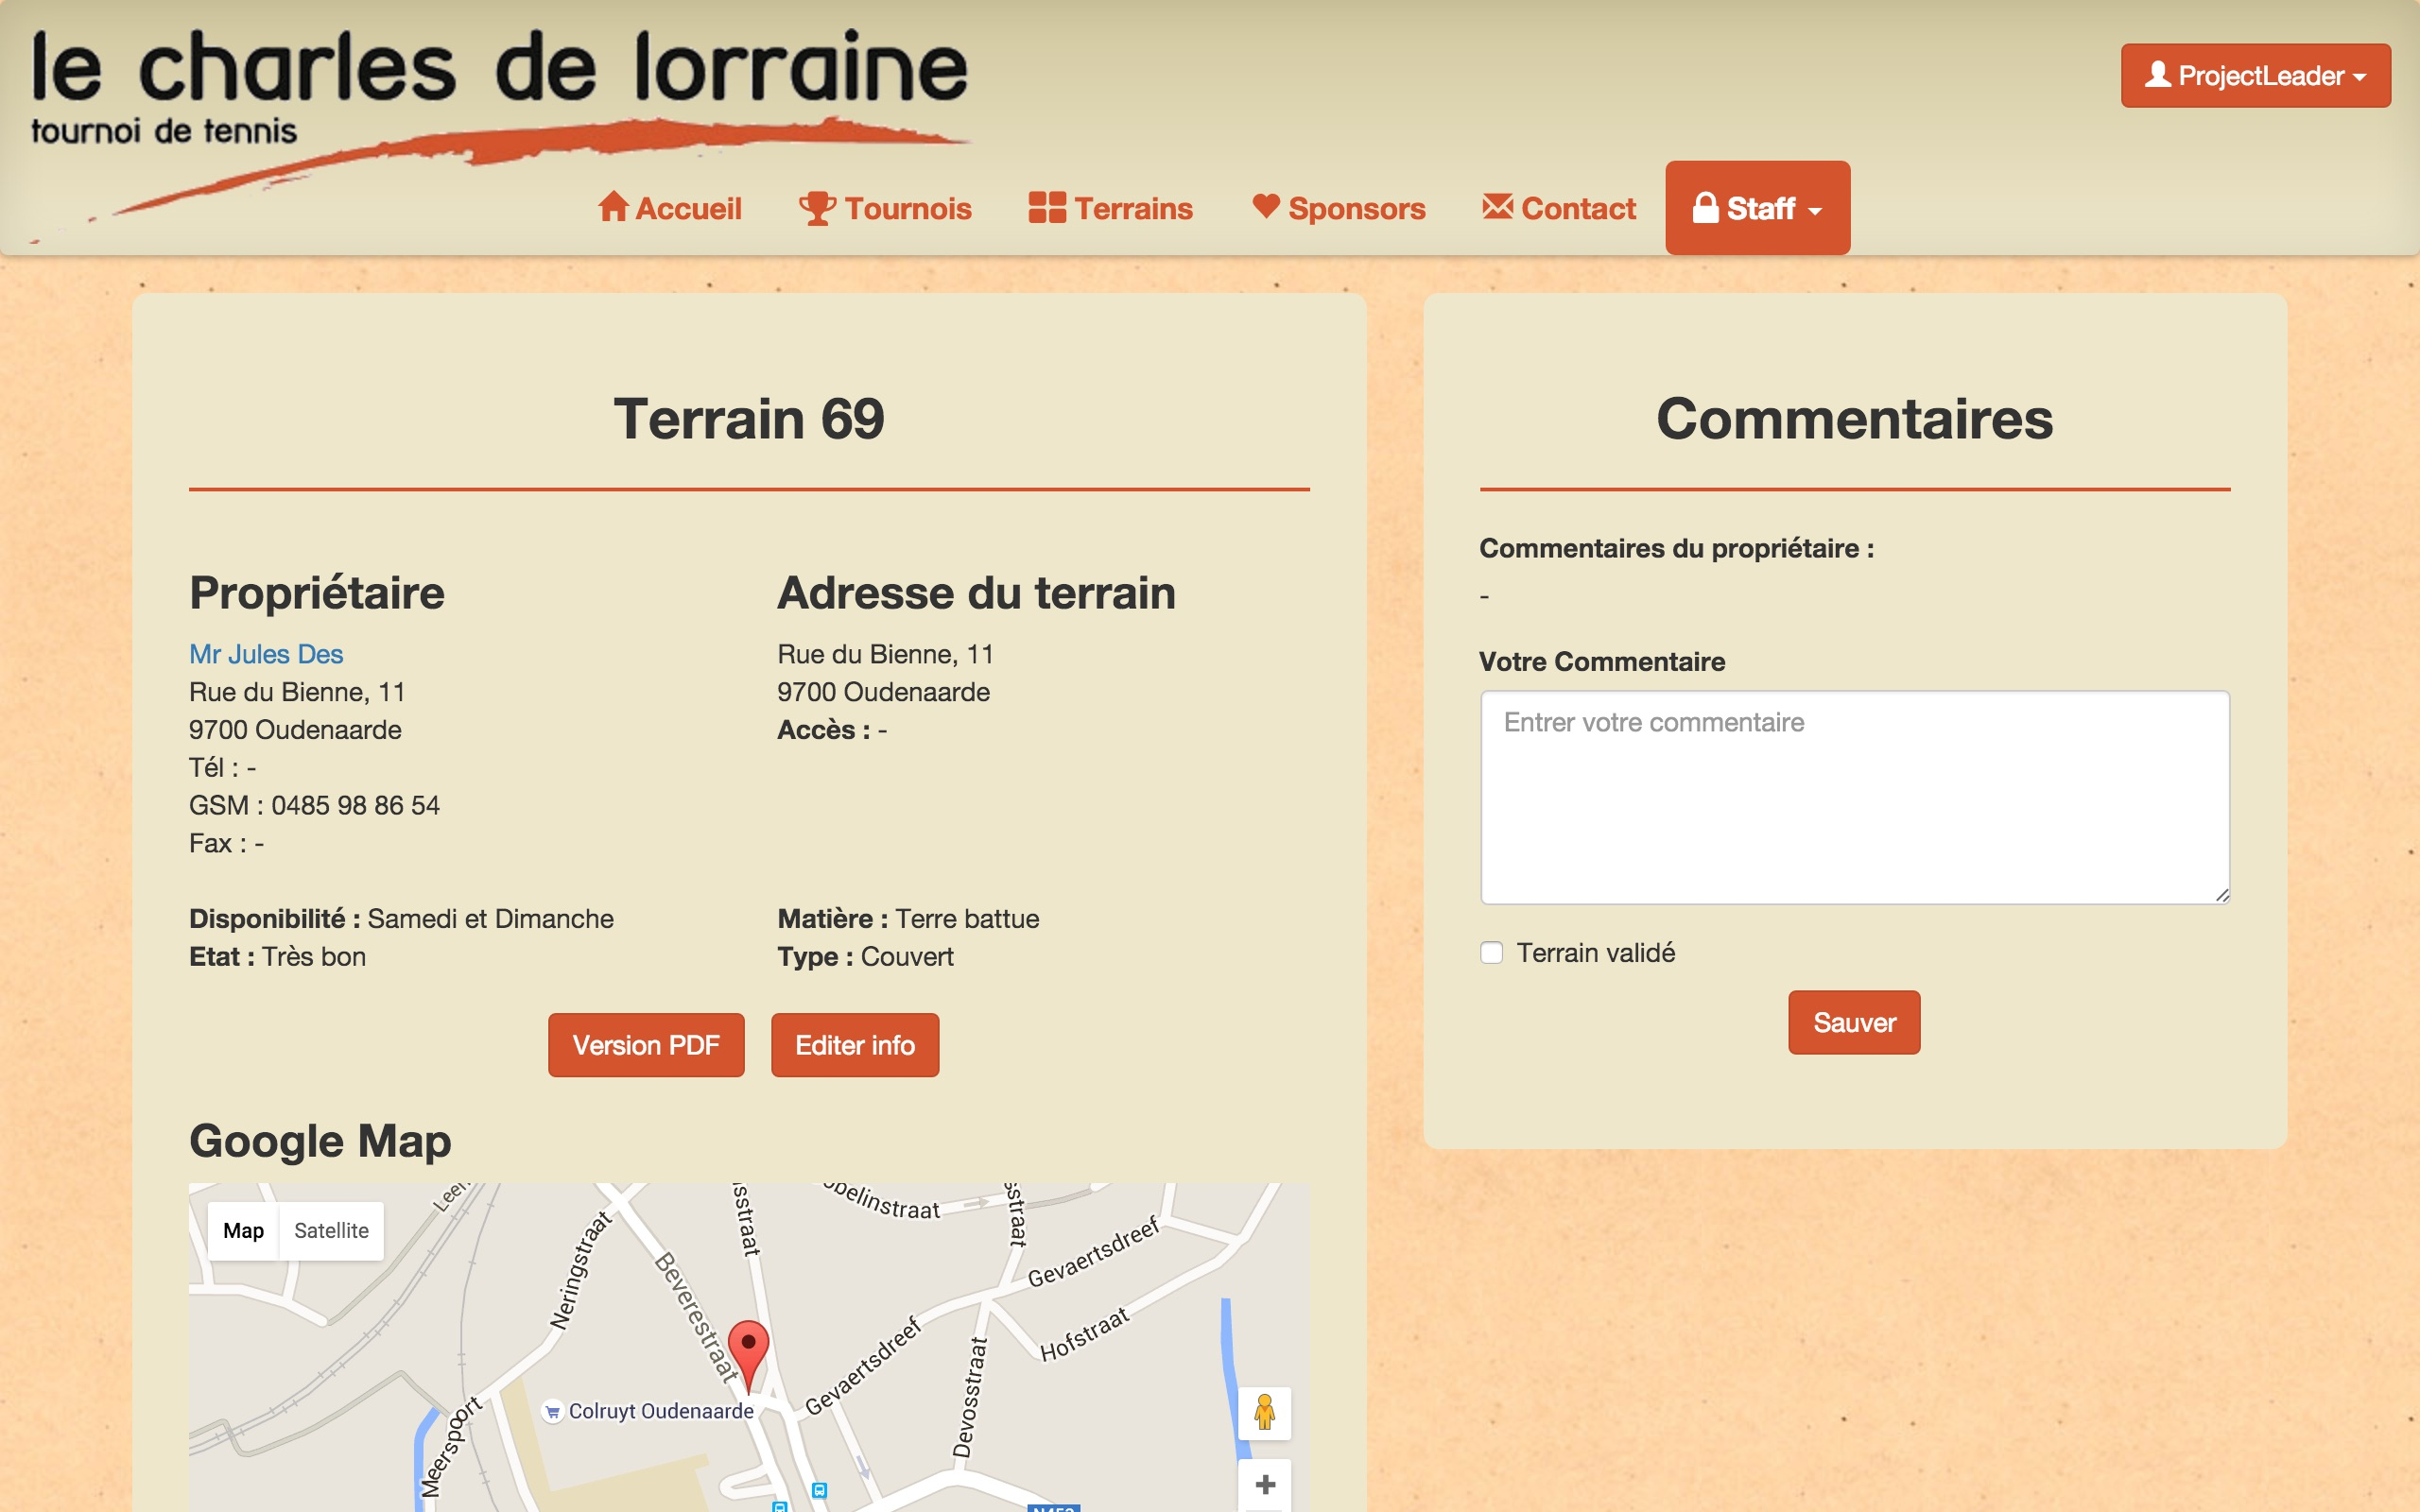
\includegraphics[scale=0.15]{user_images/staff/GererPaires/001.jpg}
\caption{Gestionnaire des paires}
\end{figure}

\subsection{Consulter une paire}

MISSING!

\subsection{Valider une paire}

Pour valider une paire, il faut accéder à la page d'une paire, comme expliqué à la sous-section "Consulter une paire".\newline

À partir de cette page, lorsque une paire n'a pas été validée, la liste déroulante "Paire validée" vaut "Non". Pour valider cette paire, il suffit de sélectionner l'entrée "Oui" dans cette liste déroulante.

\begin{figure}[H]
\centering
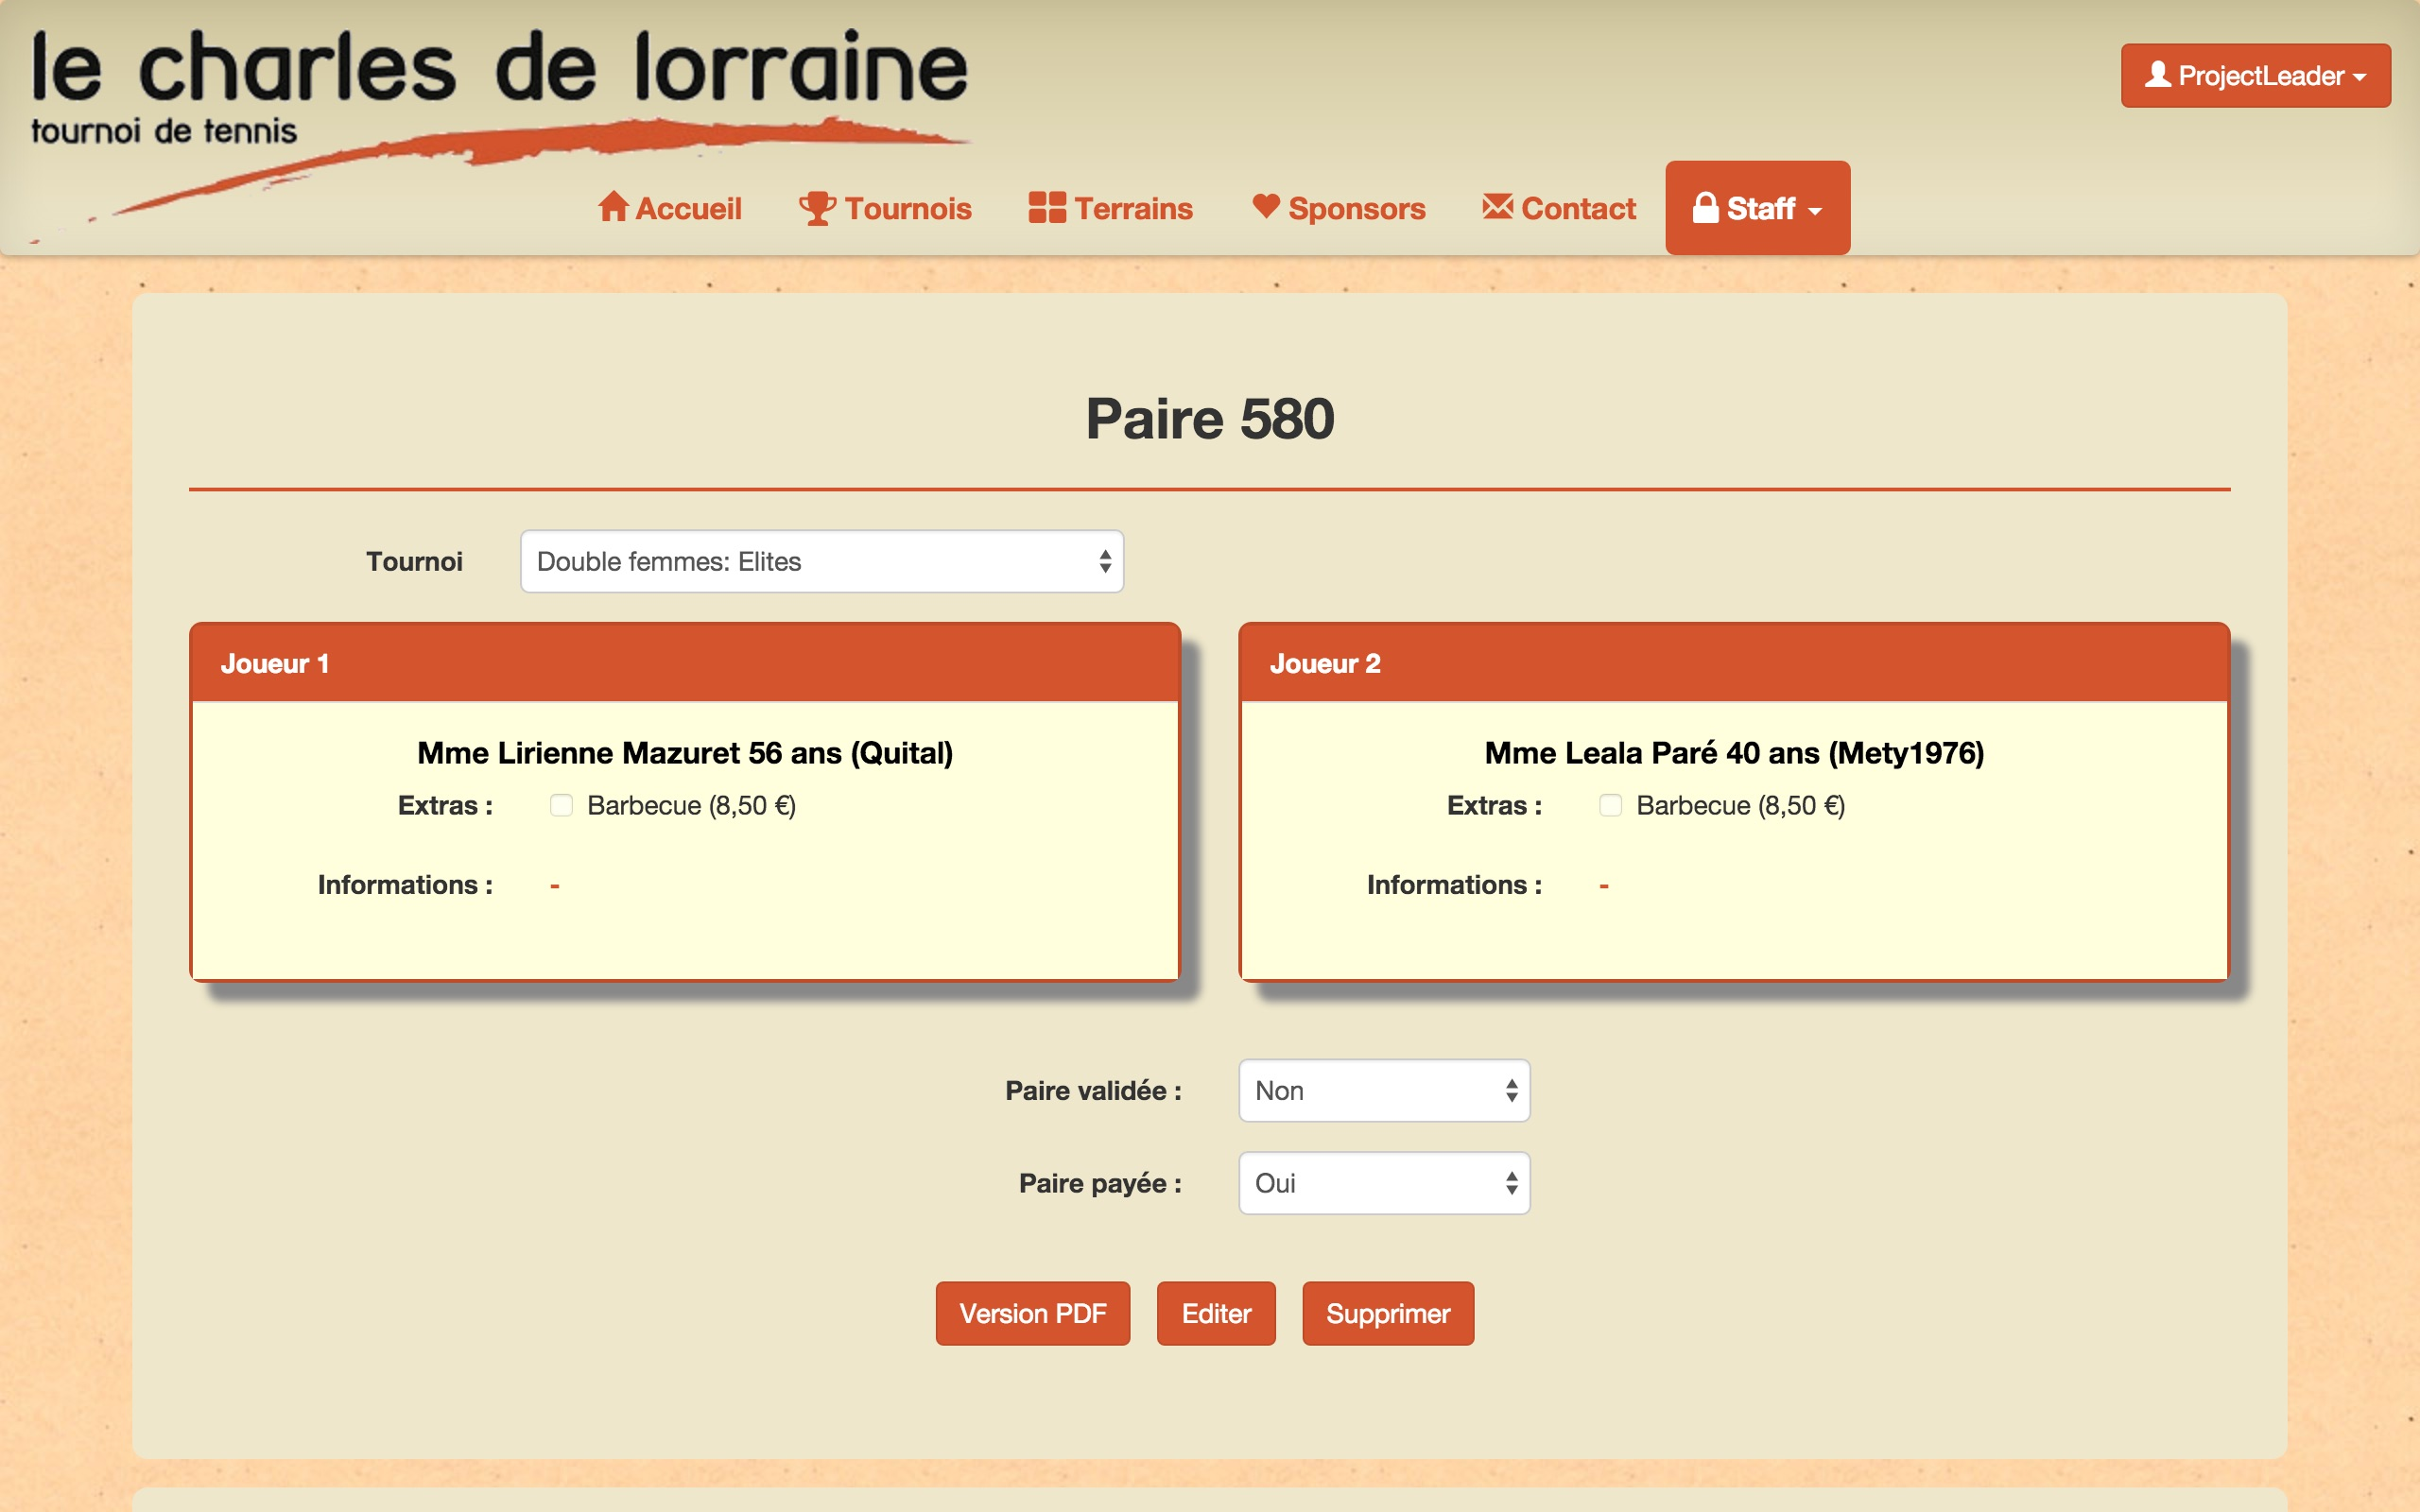
\includegraphics[scale=0.15]{user_images/staff/GererPaires/ValiderPaires/002.jpg}
\caption{Valider une paire, étape 1}
\end{figure}

Dès que l'attribut "Paire validée" vaut "Oui", confirmez le changement en cliquant sur le bouton "Editer".

\begin{figure}[H]
\centering
\includegraphics[scale=0.15]{user_images/staff/GererPaires/ValiderPaires/003.jpg}
\caption{Valider une paire, étape 2}
\end{figure}

Après avoir cliqué sur le bouton "Editer", la paire est bien validée. L'historique de la paire indique que la paire a été récemment validée.

\begin{figure}[H]
\centering
\includegraphics[scale=0.15]{user_images/staff/GererPaires/ValiderPaires/004.jpg}
\caption{Valider une paire, étape 3}
\end{figure}

Sur la page principale du gestionnaire des paires, en filtrant les paires de telle manière à avoir la paire récemment validée comme première entrée de la liste des paires, on observe que cette paire contient un marqueur vert pour la colonne "Validé", confirmant à nouveau la validation de cette paire.

\begin{figure}[H]
\centering
\includegraphics[scale=0.15]{user_images/staff/GererPaires/ValiderPaires/005.jpg}
\caption{Valider une paire, étape 4}
\end{figure}

\subsection{Supprimer une paire}

Pour supprimer une paire, il faut accéder à la page d'une paire, comme expliqué à la sous-section "Consulter une paire".\newline

Dès qu'on est sur la page de la paire, cliquez sur le bouton "Supprimer" en bas de la page pour supprimer la paire.

\begin{figure}[H]
\centering
\includegraphics[scale=0.15]{user_images/staff/GererPaires/SupprimerPaires/003.jpg}
\caption{Supprimer une paire, étape 1}
\end{figure}

Étant donné que cette action est irréversible, une boîte de dialogue demande confirmation de l'action de l'utilisateur de supprimer cette paire.

\begin{figure}[H]
\centering
\includegraphics[scale=0.15]{user_images/staff/GererPaires/SupprimerPaires/004.jpg}
\caption{Supprimer une paire, étape 2}
\end{figure}

Après confirmation de la volonté de supprimer la paire par l'utilisateur, la paire ne se trouve plus dans la liste des paires.

\begin{figure}[H]
\centering
\includegraphics[scale=0.15]{user_images/staff/GererPaires/SupprimerPaires/005.jpg}
\caption{Supprimer une paire, étape 3}
\end{figure}

En bas de la page, l'historique des modifications des paires confirme l'action récente de suppression de la paire.

MISSING FIGURE!